\documentclass{article}

\usepackage{graphicx}
\usepackage{hyperref}
\usepackage[utf8]{inputenc}
\usepackage[french]{babel}
\usepackage{float}
\usepackage{parskip}
\setlength{\parindent}{15pt}


\newcommand{\initMoney}{250'000}


\title{De Révolution à Evolution \\ Création d'un jeu vidéo sur les thèmes de l'écologie et de la transition énergétique}
\date{2017-2018}
\author{Niels Lachat, 3MG01 \\ Mentor : Patrick Rickli \\ Lycée Denis-de-Rougemont}

\begin{document}
        \pagenumbering{gobble}
        \maketitle
        \newpage

        \tableofcontents
        \newpage
        \pagenumbering{arabic}

        \section{Introduction}
        Le but de ce travail de maturité était de créer un jeu vidéo abordant les thématiques de l'environnement et de la transition énergétique. 
        Le genre du jeu de gestion a été choisi pour démontrer les principes économiques de la transition énergétique.
        Ces principes ont bien entendu été simplifiés et modélisés afin de pouvoir les intégrer dans un jeu vidéo.
        
        
        Je présenterai tout d'abord le concept sur lequel le jeu a été basé et j'expliquerai ensuite comment le joueur interagit avec le jeu.
        Je conclurai par une explication du fonctionnement de certaines parties du code du jeu.

        \section{Concept du jeu}
        \subsection{Développement du concept}
        
        Mon projet était de créer un jeu de gestion de ressources dont l'univers du jeu était aussi proche que possible de la réalité. Le joueur (incarnant le président/la présidente du monde fictif) commence sa partie au début du 18\textsuperscript{ème} siècle. Il devait être amené au fil des expériences du jeu à réaliser qu'à un certain moment, une transition énergétique était nécessaire afin d'assurer la survie de l'espèce humaine.
        
        \subsubsection{La mécanique économique}
        La mécanique économique étant la mécanique principale de jeu, il était primordiale qu'elle soit bien pensée.
        Plusieurs mécaniques économiques m'ont parues intéressantes mais je n'en ai retenue qu'une seule pour les raisons décrites ci-dessous.
        
        
        La première alternative consistait à avoir deux types de centrales: des centrales produisant de l'énergie (centrales à charbon, barrages hydroélectriques, centrales nucléaires, etc...) et d'autres produisant des ressources (usines de textile, forges, champs, etc...). Le joueur installerait des centrales énergétiques pour produire de l'énergie permettant de faire fonctionner ses centrales produisant des ressources. Ainsi, un cycle économique se créerait. 
        Deux raisons m'ont convaincu de ne pas choisir cette alternative. Premièrement, l'idée ci-dessus ne transmettait pas le message que je voulais transmettre: en effet, ce n'est pas ce que l'on produit et ce que l'on consomme qui pose un problème, c'est la façon dont nous le faisons. Ce qui m'amène à la deuxième raison m'ayant fait renoncer à cette alternative: la complexité des mécaniques de jeu et par conséquent du code.
        
        
        La deuxième alternative était basé sur deux types de centrales: les centrales de production de ressources énergétiques (mines, puits de pétroles, etc...) et les centrales de production d'énergie (citées ci-dessus). Le joueur devrait trouver un bon équilibre entre les ressources énergétiques qu'il produirait et les centrales énergétiques qui consomment ces ressources.
        Cette alternative aurait pu être intéressante du point de vue du joueur mais elle était également trop compliquée à intégrer dans le jeu et ne reflétait pas non plus l'idée que je voulais transmettre dans mon jeu (les centrales de production de ressources énergétiques n'apportant pas beaucoup à la réflexion).
        
        
        J'ai donc opté pour la troisième alternative qui consiste à n'avoir qu'un seul type de centrales: les centrales de production d'énergie. Ainsi, le joueur choisit où il installe ses centrales et celles-ci produisent de l'énergie qui est convertie directement en mondios (nom de la monnaie du jeu). Il peut ainsi acheter de nouvelles centrales avec l'argent qu'il obtient.
        
        \subsubsection{Le personnage incarné par le joueur}
        Je me suis également posé la question de savoir quel personnage le joueur devrait incarner. Dans un premier temps m'est venu l'idée que le joueur pourrait être un riche patron d'une multinationale. Cependant cela impliquait que c'était du ressort des multinationales d'assurer ou non la transition énergétique et d'effectuer des actions en faveur de l'écologie, ce qui est en tout cas partiellement faux. Cette possibilité excluait également le joueur, qui ne se sentait que très peu concerné par la problématique.
        
        
        L'autre possibilité était donc que le joueur incarne le président/la présidente du monde. Cette option a l'avantage d'expliquer le pouvoir immense qu'a le joueur et de montrer que n'importe qui peut agir pour le bien de la planète.
        Un inconvénient de ce choix est que cela éloigne le monde du jeu de la réalité car le monde n'est évidemment pas gouverné par un président mondial. Cette alternative a tout de même été choisie pour simplifier la narration et le concept.
        

		\subsubsection{La monnaie du jeu}
		Une question qui s'est posée assez rapidement dans le développement de l'idée du jeu était celle du choix de la monnaie du jeu. J'ai d'abord pensé à utiliser une monnaie réelle mais la question des échelles des prix des objets du jeu m'a fait douter de ce choix. En choisissant une monnaie fictive, j'avais le choix de fixer les prix que je voulais car on ne pourrait avec des prix réels.
		J'ai donc choisi de créer les \textit{Mondios}, monnaie universelle de la planète (voir figure \ref{fig:mondiosLogo}).
		
		
		\textit{Note: }L'affichage de l'argent est toujours effectué en utilisant les préfixes du Système international d'unités pour réduire l'espace que celui-ci prend sur l'écran (par exemple 150'200 sera affiché comme 150.2k)
		\begin{figure}[H]
                \centerline{
\includegraphics[scale=.5]{../images/mondiosLogo}}
                \caption{Icône de la monnaie du jeu: les \textit{Mondios}}
                \label{fig:mondiosLogo}
        \end{figure}		
		
        \subsection{Concept final}
        Vous êtes en 1800, au début de la révolution industrielle. Vous venez d'avoir été élu président(e) de la planète. Votre but: mener la planète à travers la Révolution industrielle et assurer la transition énergétique afin de ne pas arriver à un point critique du réchauffement climatique. Le jeu s'achève soit si vous avez dépassé une température critique du réchauffement climatique (jeu perdu) ou si vous avez atteint l'année 2100 (jeu gagné).
        L'action principale du joueur consiste à gérer les centrales énergétiques présentes sur sa planète.

        \section{Le jeu}
        \subsection{Interaction du joueur}
		Dans cette section, j'expliquerai comment le joueur peut interagir avec le jeu en présentant les éléments de l'écran principal, les différents onglets du jeu, la vue des régions et comment jouer au jeu.        
        
        \subsubsection{Les éléments de l'écran principal}
		L'écran principal du jeu comporte plusieurs éléments dont je vais expliquer l'utilité ci-dessous (voir à chaque fois la figure \ref{fig:worldView}).
		
		\begin{itemize}
			\item \textbf{L'argent du joueur} (en mondios) est affiché dans le coin en haut à gauche de l'écran.
			\item \textbf{L'année de jeu} est affichée en haut au centre de l'écran. Les flèches à gauche et à droite de l'année permettent de ralentir (flèche gauche) ou d’accélérer (flèche droite) le déroulement du temps du jeu.
			\item \textbf{Le bouton plein écran} affiché en haut à droite de l'écran permet d'activer ou de désactiver le plein écran.
			\item \textbf{L'onglet de recherche} est accessible via le bouton 'Recherche' situé en-dessous du bouton plein écran. Son utilité est expliquée dans la section \ref{onglets}.
			\item  \textbf{L'onglet de statistiques} est accessible via le bouton 'Statistiques' affiché en-dessous du bouton 'Recherche'. Son utilité est également expliquée dans la section \ref{onglets}.
		\end{itemize}
		
		\begin{figure}[H]
                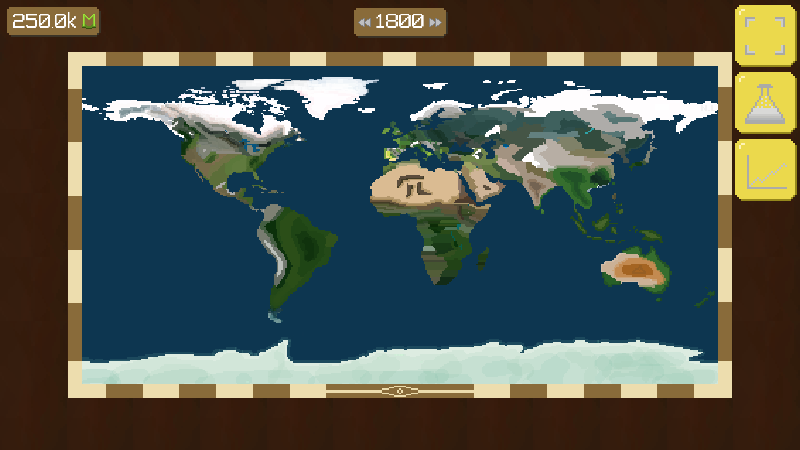
\includegraphics[width=\linewidth]{../images/worldView}
                \caption{Ecran principal du jeu}
                \label{fig:worldView}
        \end{figure} 
		
		\subsubsection{Les onglets du jeu} \label{onglets}
		Les menus du jeu sont affichés sous la forme d'onglets (qui représentent un journal).
		Il y a 3 onglets qui sont sous cette forme de journal: l'onglet de recherche, l'onglet des statistiques et l'onglet d'achat de centrales.
		Tous les onglets sont construis sur le même modèle, seul leur contenu change. Ainsi, chaque onglet comporte un titre (en haut au centre), un bouton permettant de fermer l'onglet (en haut à droite), trois sections (au centre), un numéro de page (en bas au centre) et des flèches pour changer de page (en bas à gauche et à droite).
		
		
		\textbf{L'onglet de recherche} affiche les centrales énergétiques dans lesquelles le joueur peut investir des mondios (en appuyant sur le bouton vert où le prix de l'investissement est affiché) pour augmenter la probabilité qu'il les débloquera.
		
		\begin{figure}[H]
                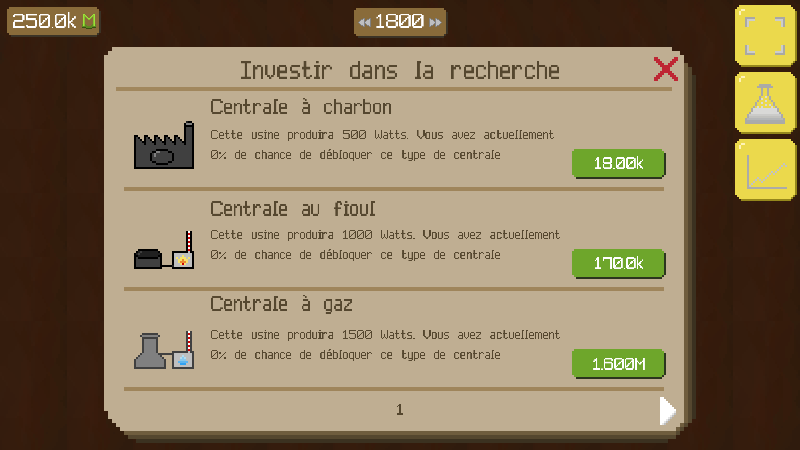
\includegraphics[width=\linewidth]{../images/recherche}
                \caption{Onglet de recherche}
                \label{fig:research}
        \end{figure}
        
        
        \textbf{L'onglet des statistiques} affiche les différentes statistiques de jeu. 
		
		\subsubsection{La vue des différentes régions}
        
        \subsubsection{Comment jouer}
        Le joueur commence par devoir choisir de jouer avec ou sans tutoriel pour lui expliquer les bases du jeu (voir figure \ref{fig:mainMenu}). 
        
        \begin{figure}[H]
                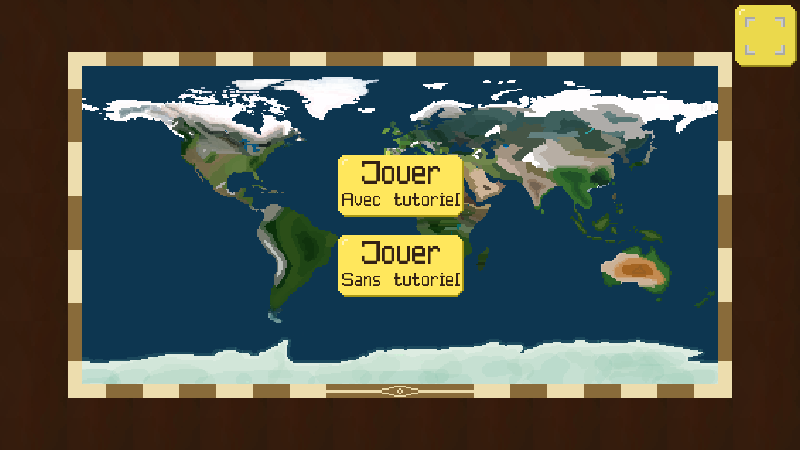
\includegraphics[width=\linewidth]{../images/mainMenu}
                \caption{Menu principal du jeu}
                \label{fig:mainMenu}
        \end{figure}
        
        
        S'il choisit de suivre le tutoriel, il sera guidé dans le jeu avec le personnage de Conseil qui lui expliquera le fonctionnement de tous les éléments du jeu et le but de la partie.
        
        
        Lorsqu'il commence une partie, le joueur commence avec \initMoney ~ Mondios. Il devra d'abord utiliser cet argent dans l'onglet 'Recherche' (voir figure \ref{fig:research}) qui lui permettra de débloquer une centrale énergétique. Après avoir suffisamment investit dans un type de centrale et attendu un certain moment (les centrales ne peuvent se débloquer qu'à chaque passage d'année), le type de centrale se débloque.
        \

        \subsection{Fonctionnement du jeu}
        
        \section{Conclusion}
        \subsection{Ce que j'aurais aimé rajouter dans le jeu}

        

        Figure \ref{fig:mainMenu}

        \href{https://www.latex-tutorial.com/tutorials/pgfplots/}{Lien vers le tuto}



\end{document}
